\documentclass[14pt, letterpaper, twoside]{article}
\usepackage[hmarginratio=1:1, margin=1in]{geometry}
\usepackage{fancyhdr}
\usepackage{titlepic}
\usepackage{pdfpages}
\usepackage[colorlinks=true, urlcolor=blue, linkcolor=blue]{hyperref}
\usepackage{graphicx}
\usepackage[mmddyyyy]{datetime}
\usepackage{fancyhdr}
\setlength{\parskip}{2mm}
\setlength{\parindent}{0mm}
\setcounter{secnumdepth}{5}
\setcounter{tocdepth}{5}
\usepackage{setspace}
\pagestyle{fancy}
\fancyfoot{}


\titlepic{
\includegraphics[width=2in]{logo.png}}
\title{\textbf{Name Our Lion Moscot\\ What's My Mame?}
    \begin{spacing}{1.5} 
    This educational activity not only accomplishes the goal of naming our school's lion mascot but also imparts valuable life skills, character development, and a strong sense of belonging and unity within school community. It encourages students to become active participants in shaping our school's identity and 			culture, emphasizing the importance of values, teamwork, and leadership. 
    \end{spacing}}
\date{}
\author{September 11, 2023}


% Cover Page
%%%%%%%%%%%%%%%%%%%%%%%%%%%%%%%%%%%%%%%%%%%%%%%%%%%%%%%%%%%%%%%%%%%%%%%%%%%%%%%%%%%%%%%%%%%%%%%%%%
\begin{document}

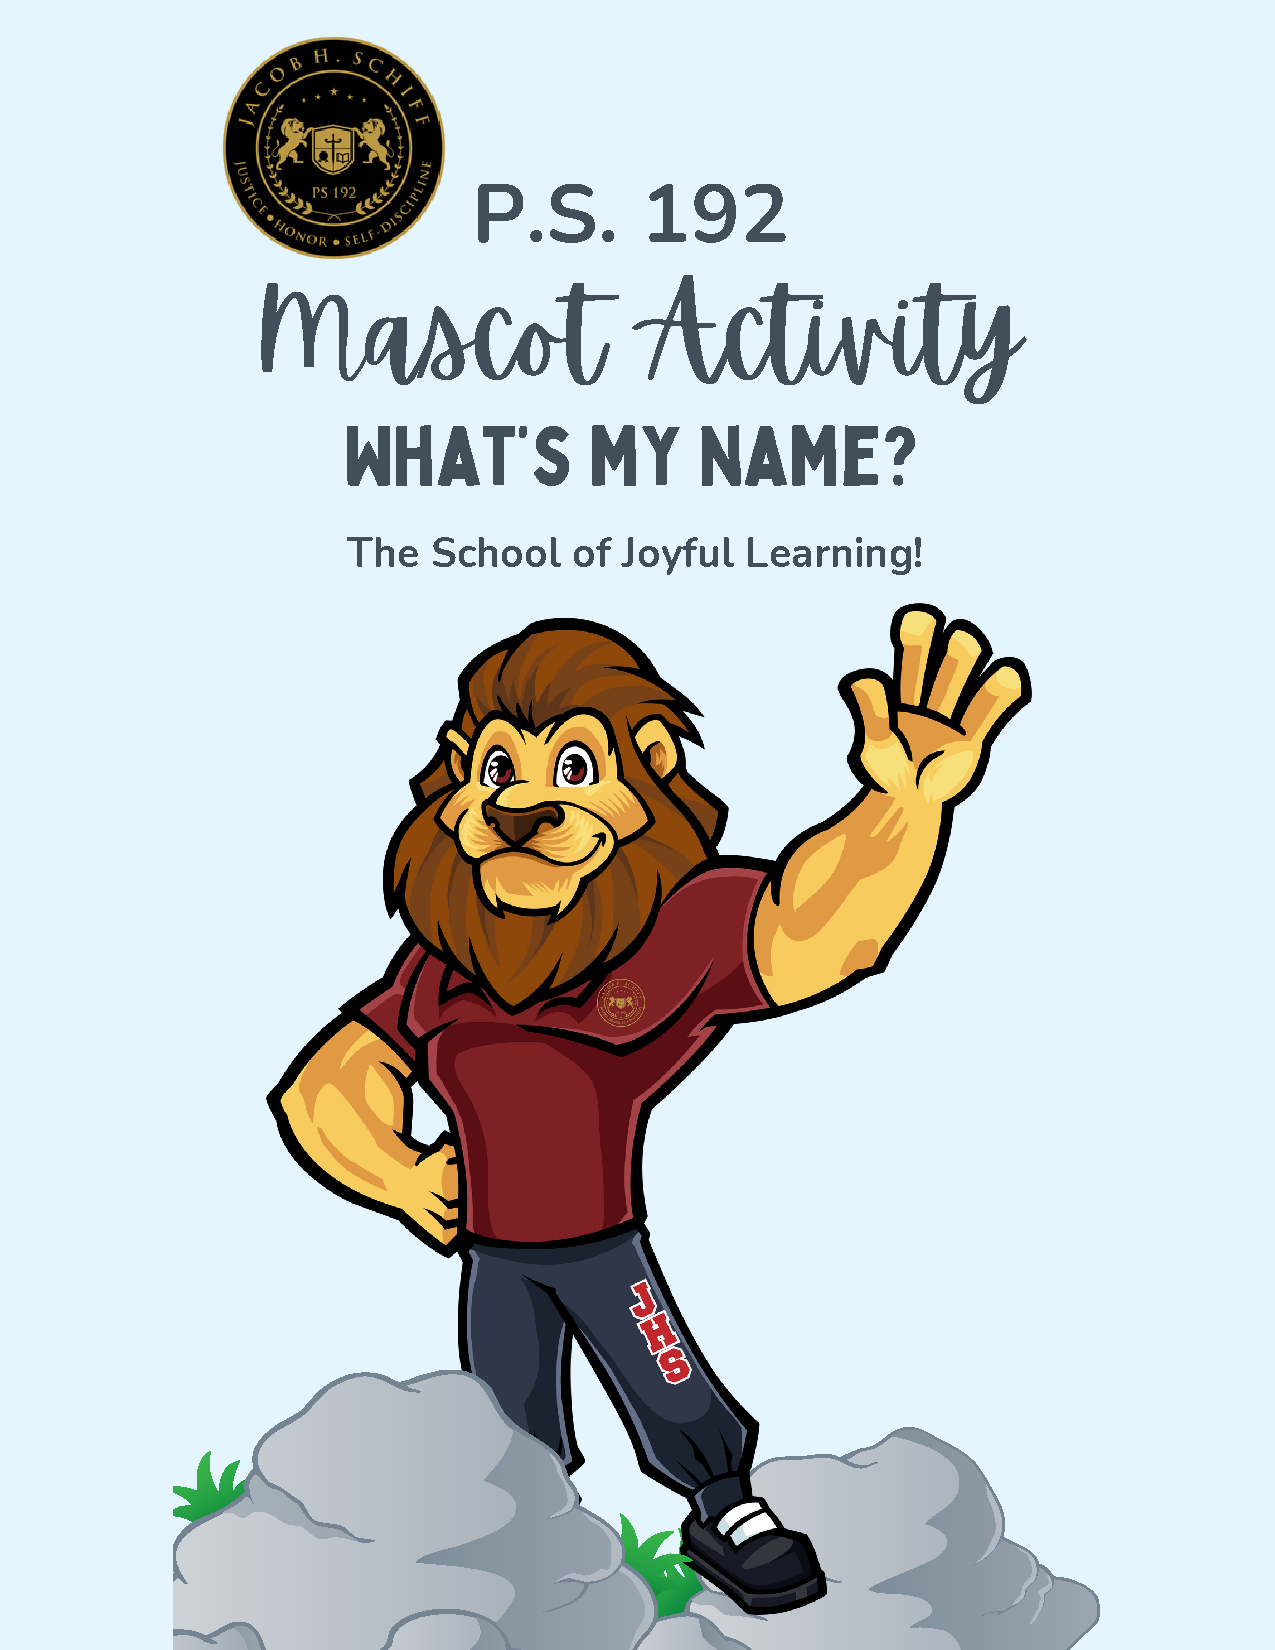
\includepdf[pages=1,fitpaper]{ps192-mascot}

\begin{titlepage}
  \maketitle 
  \thispagestyle{empty} 
\end{titlepage}

\pagenumbering{arabic}
\pagestyle{headings}

\fancyhf{}
\fancyhead[L]{\textit{What's my name?}}
\fancyhead[R]{\thepage}
\fancyfoot[C]{The School of Joyful Learning!}
\pagestyle{fancy}
\renewcommand{\footrulewidth}{1 px}

% TOC
%%%%%%%%%%%%%%%%%%%%%%%%%%%%%%%%%%%%%%%%%%%%%%%%%%%%%%%%%%%%%%%%%%%%%%%%%%%%%%%%%%%%%%%%%%%%%%%%%%

\newpage
\tableofcontents
\thispagestyle{empty}
\newpage


\section{Activity Description}

	"Name the Lion Mascot is an engaging activity designed for emphasizing and reinforcing the school's core values of Justice, Honor, and Self-discipline. In addition, the activity fosters a sense of unity, collaboration, and leadership within the school community.
	
	\subsection{What Kids Will Learn:}
	\begin{itemize}
	\item What Kids Will Learn:
		\begin{itemize}
		\item Core Values: 
			\begin{itemize}
			\item Students will gain a deeper understanding of the school's core values—justice, honor, and self-     			discipline—through discussions and brainstorming sessions. They will learn to connect these values 					with real-life examples and how they shape our school's culture.
			\end{itemize}
		\item Creativity and Collaboration: 
			\begin{itemize}
			\item The activity encourages students to work together in groups to brainstorm and propose names for the lion mascot. They will learn to combine their creative ideas, compromise, and make collective decisions, promoting teamwork and collaboration. Explicitly model, rehearse the K-2 or 3-5 Collaborative Discussion guide and the protocol for working in groups.
			\end{itemize}
		\item Communication Skills:
			\begin{itemize}
			\item When presenting their chosen lion names to the class, students will develop their communication 					skills by articulating their ideas and explaining how the names relate to the school's values. This 					helps improve their ability to express themselves clearly and persuasively. Explicitly model and rehearse the K-2 or 3-5 Discussion Guide.
			\end{itemize}
    		\item Democracy and Voting: 
    			\begin{itemize}
    			\item The voting process teaches students about democratic decision-making. They will experience the 					importance of individual voices and the collective will of the community in choosing a mascot name.
			\end{itemize}
		\item Leadership Principles:
			\begin{itemize}
			\item During the leadership discussion, students will explore the qualities and responsibilities of leaders in promoting the core value of Justice (unity and collaboration.) Students will understand that leadership isn't limited to individuals but can be collective and inclusive.
			\end{itemize}
     	\item Sense of Belonging:
    			\begin{itemize}
    			\item Students will pledge their commitment to the chosen mascot name. This instills a sense of belonging and ownership in their school community.
    			\end{itemize}
		\item Mascot Symbolism:
			\begin{itemize}
			\item Students will learn about the symbolism of a mascot and its role in representing their school's 					identity. They will see how the chosen name can inspire pride and a strong sense of identity among 					students.
			\end{itemize}
		\item Long-Term Engagement:
			\begin{itemize}
			\item The ongoing implementation of the mascot name in school activities and events will reinforce the sense of community, and we must ensure that these lessons and events are carried forward throughout the school year.
			\end{itemize}
		\end{itemize}
	\end{itemize}
\section{Title: "Name Our Mascot"}

	\subsection{Lesson Objective:}

	The objective of this educational activity is to engage our students in a collaborative and 				creative process to name our school's lion mascot. Through this activity, students will not only learn about the school values of justice, honor, and self-discipline but also develop a sense of unity, collaboration, and 	leadership within our school community. Read aloud and analyze the objective of the lesson, and co-create the I can statement with students.
	
	Standards: 
	
	CASEL 13: Relationship Skills: Learners will be able to use active listening and assertive, clear communication when expressing thoughts and ideas.
	
	CASEL 16: Relationship Skills: Learners will be able to work cooperatively and productively in a group and overcome setbacks and disagreements.

	\begin{itemize}
	\item Materials Needed:
		\begin{itemize}
    		\item Coloring materials (crayons, colored pencils, markers)
    		\item Large poster paper
    		\item Sticky notes or index cards
    		\item Ditigital and audible countdown clock
    		\item Computer and projector (optional)
    		\item Prize for the winning name (e.g., certificate, Lunch with the Pricipal and teacher, 1 period of recess)
		\end{itemize}
	\item Lesson Development : Activity Steps
		\begin{itemize}
    		\item Introduction (10-15 minutes):
    		
    		Begin by gathering all the students in the area(sitting in a circular or "U" shape. Explain the purpose of the activity to name the school's lion mascot. Emphasize that the chosen name should reflect the school's core values of justice, honor, and self-discipline. Discuss the importance of unity, collaboration, and leadership 			within the school community. Explicitly model, discuss and rehearse the the role of the speaker and the role of the listener. Co-create the anchor chart.
		\item Brainstorming (5-10 minutes):
		\begin{itemize}
    		\item Break the students into smaller groups, ensuring that each group has a mix of levels and 						personalities 		to encourage collaboration. Give each group a large sheet of poster paper and markers. Ask them to brainstorm lion names that align with the school values. Encourage creativity and teamwork. Teacher canvasing the room to document individual and team trends and patterns of teams working collaborative using the collaborative discussion guide (role of the speaker/listener) to anchor feedback and record individual/group noticings.
    		\end{itemize}
    		\item Presentations (15 minutes):
		\begin{itemize}
    		\item Each group will present their chosen lion name and explain why it reflects justice, honor, and self-	discipline. Use the chart paper or a google doc to write down the names and rationales. Discuss the qualities of each proposed name and how it relates to the school's values. (3 minutes per group.)
    		\end{itemize}
		\item Voting (10 minutes):
		\begin{itemize}
    		\item Give each student sticky notes or index cards and ask them to vote for their favorite lion name from the 				presented options. They can write the name on the card or stick the sticky note next to the name on the board.
    		\end{itemize}
		\item Lesson Wrap-Up: Leadership Discussion (10 minutes):
		\begin{itemize}
    		\item While the votes are being counted, lead a discussion about leadership and how leaders can inspire 				unity and collaboration. Emphasize the role of the speaker and the role of the listener. Discuss the role 				of the mascot in representing the school and fostering a sense of community.
    		\end{itemize}
    		\item Announcement of the Winning Name (5 minutes):
		\begin{itemize}
    		\item Announce the winning lion name that received the most votes. This is the name that will be entering 				the school-wide contest for families, staff and students to vote to select the final moscot name. 						Celebrate the winning group and the name they chose. Award a prize to the group: certificate, lunch with the teacher, a no homework card.
    		\end{itemize}
		\item Unity Pledge (5 minutes):
		\begin{itemize}
    		\item To conclude the activity, lead a unity pledge where all students, including those not in the winning 		group, promise to embrace the chosen mascot's name and its values, fostering unity and collaboration 					within the school.
    		\end{itemize}
		\item Name Implementation (ongoing):
		\begin{itemize}
    		\item Application of objective learned: Incorporate the newly chosen lion mascot name into school 						activities, events, and materials, reinforcing the values of justice, honor, and self-discipline, as well 				as the sense of unity and collaboration among students. 
    		\end{itemize}
    		
Teacher Final Summary: Today we learned not only to use our creativity but also learned important values such Justice, Honor and Self-displine (based on your observations, select one example of each of  core value. "We showcased Justice by... We exhibited honor by... We accomplished self-disciple when...) and a sense of belonging within our school community, all while promoting leadership and teamwork. Draft summary in chart paper to model a lesson reflection (select a small chart tablet to draft your daily teacher lesson reflection (summary.) These summaries will be use as relection exemplars for you to discuss and co-create the criteria of "What Makes a Good Lesson Reflection." Chart will be displayed and information will be added for the next two weeks to co-create the final criteria for a reflection prompt.
		\end{itemize}
    
	\end{itemize}

\end{document}
